\chapter{The W boson}
    This chapter is dedicated to the electroweak sector of the \gls{sm} and in particular to the W boson. The aspects of the theoretical modelling of the W boson production and kinematic distributions are discussed. The last section mentions previous measurements of the W boson transverse spectrum and speculates about the target precision for its direct measurement. 
    	\section{The motivation for the W mass measurement}    
        Being one of the cornerstones of the \gls{sm}, the W boson is tightly connected to the other parameters of the theory. In the leading order of the perturbation theory the W mass depends only on the electroweak parameters~\cite{Awramik}:
        \begin{equation}
        M_W=\sqrt{\frac{\pi \alpha_{EM}}{\sqrt{2}G_F}}\frac{1}{\sin{\theta_W}},
        \end{equation}
        where $G_F$ stands for the Fermi constant, $\alpha_{EM}\approx\frac{1}{137}$ is the electromagnetic coupling constant and $\sin{\theta_W}$ is the Weinberg angle (see \ref{sec:symmetry_breaking}). The factor $\sqrt{\frac{\pi \alpha}{\sqrt{2}G_F}} \approx 40$ GeV sets the lower bound for the possible W mass. Higher order corrections enter the equation in the following way:
        \begin{equation}
        M_W=\sqrt{\frac{\pi \alpha}{\sqrt{2}G_F}}\frac{1}{\sin{\theta_W}}(1+\Delta r),
        \end{equation}
        where $\Delta r $ contains the sum of all possible radiative corrections and depends also on other parameters of the \gls{sm}, first of all on top quark and Higgs boson masses. The correction term is also sensitive to possible \gls{bsm} effects.
        \begin{figure}
        	\label{fig::mw_cor}
        	\centering
        	\feynmandiagram [horizontal=a to b, layered layout] {
        		i1 -- [boson, edge label = \( W \)] a,
        		a -- [scalar, half left, , edge label = \( H \)] b,
        		a -- [boson] b,
        		b -- [boson, edge label = \( W \)] f1,
        	};
        		\;  \; \; \; 
        	\feynmandiagram [horizontal=a to b,  layered layout, baseline=(b)] {
        		i1 -- [boson, edge label = \( W \)] a,
        		a -- [fermion, half left, , edge label = \( t \)] b,
        		b -- [fermion, half left, , edge label = \( \bar b \)] a,
        		b -- [boson, , edge label = \( W \)] f1,
        	};
        	\caption{ Next-to-leading order diagrams for W boson propagator containing contributions from heavy quarks and the Higgs boson.}
        \end{figure}
    As it was mentioned in Chapter 1 the mass of the W boson is one of the input parameters of the \gls{sm}, so the predictions of the theory directly depend on how precisely we know the value of the boson mass. On the other hand, we can theoretically constrain the value of the W boson mass assuming the already known values of the other \gls{sm} parameters. Figure \ref{fig::w_values} demonstrates that the uncertainty on the theoretical estimate for the W boson mass is about two times lower than that of the best available experimental measurement. This motivates the effort for a more precise experimental measurement in order to test the consistency of the \gls{sm}. Should the improved measurement reveal the inconsistency of the Standard Model - it would also allow to reveal viable \gls{bsm} theories. 
    	\begin{figure}[htbp]
    	\begin{subfigure}[t]{0.48\textwidth}
    		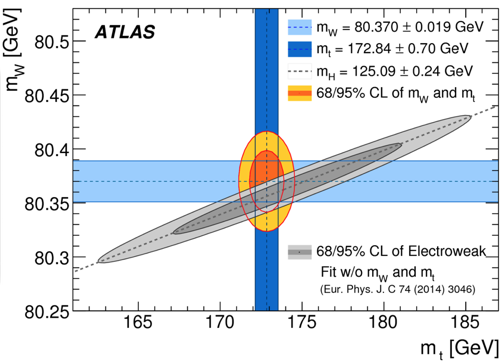
\includegraphics[width=\textwidth,keepaspectratio]{mw2.png}
    		\caption[Side view]{W mass constraint from the global electroweak fit.}
    		\label{fig::w_constraint}
    	\end{subfigure}
    	\hfill
    	\begin{subfigure}[t]{0.48\textwidth} 
    		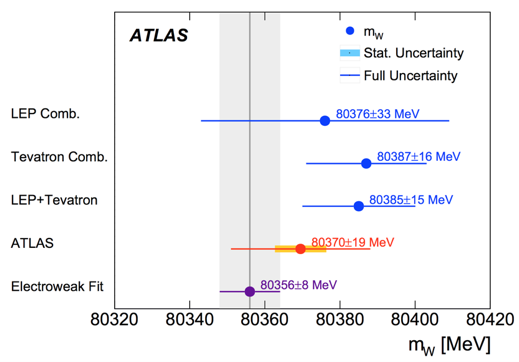
\includegraphics[width=\textwidth,keepaspectratio]{mw1.png}
    		\caption[Transverse view]{Available W mass measurements.}
    		\label{fig::w_measurement}
    	\end{subfigure}
    	\caption{W mass measurements and predictions~\cite{wboson}.}
    	\label{fig::w_values}
    \end{figure}
        \section{Massive boson production at hadron colliders}
		Hadron colliders provide a fruitful environment for the production and study of massive electroweak bosons - all of them were discovered at hadron colliders. Hadron colliders allow to achieve much higher centre-of-mass collision energy and luminosity comparing to their lepton counterparts. At the same time precision measurements at hadron colliders demand much deeper theoretical understanding of different aspects of the \gls{sm}. \\
		The main theoretical complication of proton-proton colliders lies in the fact that contrary to leptons, protons are complex objects. This raises the following problems:
		\begin{itemize}
		\item A proton-proton collision is in the general case a many-body problem. The accompanying low-energy QCD processes can not be described from the first principles and introduce additional complications for the precision measurements.
		\item The initial energy of the whole proton is known with good precision, but we don't know how this energy is distributed among the proton constituents. The absence of a consistent theory for the QCD vacuum does not allow to describe the initial states of the proton constituents.
		\item We know that the proton consists of three valence quarks that have trivially non-vanishing PDFs and interact through gluons. In the course of these interactions all flavours of quarks (called sea quarks) are appearing through radiative mechanisms. The contribution of these sea quarks to the scattering cross-section must also be taken in account.  
		\end{itemize}
		In order to attack these problems and obtain accurate predictions for the proton-proton collisions it is necessary to take into account the asymptotic freedom that QCD demonstrates at short distances or high energies. At a certain energy scale of the momentum $Q$, transferred during the collision, we can assume that the interacting parts of the proton are asymptotically free and neglect the interaction with the rest of the proton. The factorization occurs only if the transferred momentum $Q\gg \Lambda_{QCD}$ is large, and that is why these processes are called "hard". The physical conditions of the hard processes allow to use the perturbative QCD formalism, since at large energy scale the strong coupling constant $\alpha_s$ becomes small. Processes with lower energy scale of the transferred momentum are called "soft" and do not allow to use the perturbative QCD formalism. As it was mentioned in Section 1, a lot of things in the low-energy non-perturbative sector of the QCD are still unclear. \\
		The production of massive vector bosons occurs during hard processes, however, precise measurements at hadron colliders require understanding of both hard and soft QCD regimes. It is common that the hard scattering of the proton constituents is accompanied by a soft scattering of the remaining proton parts. This forms what is called \textit{underlying event} and also must be taken into account. 
		    	\begin{figure}[htbp]
			\begin{subfigure}[t]{0.42\textwidth} 
				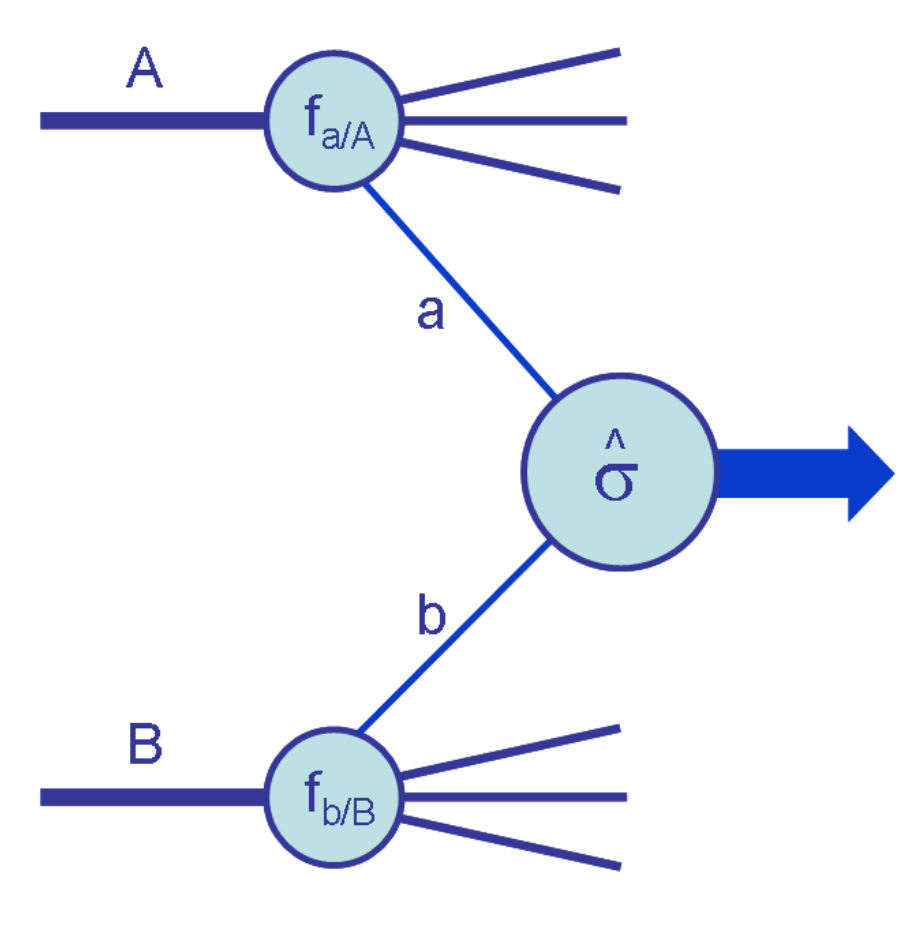
\includegraphics[width=\textwidth,keepaspectratio]{hard_scattering.png}
				\caption[Transverse view]{Hard scattering diagram~\cite{hard_interactions}.}
				\label{fig::hs}
			\end{subfigure}
			\begin{subfigure}[t]{0.52\textwidth}
				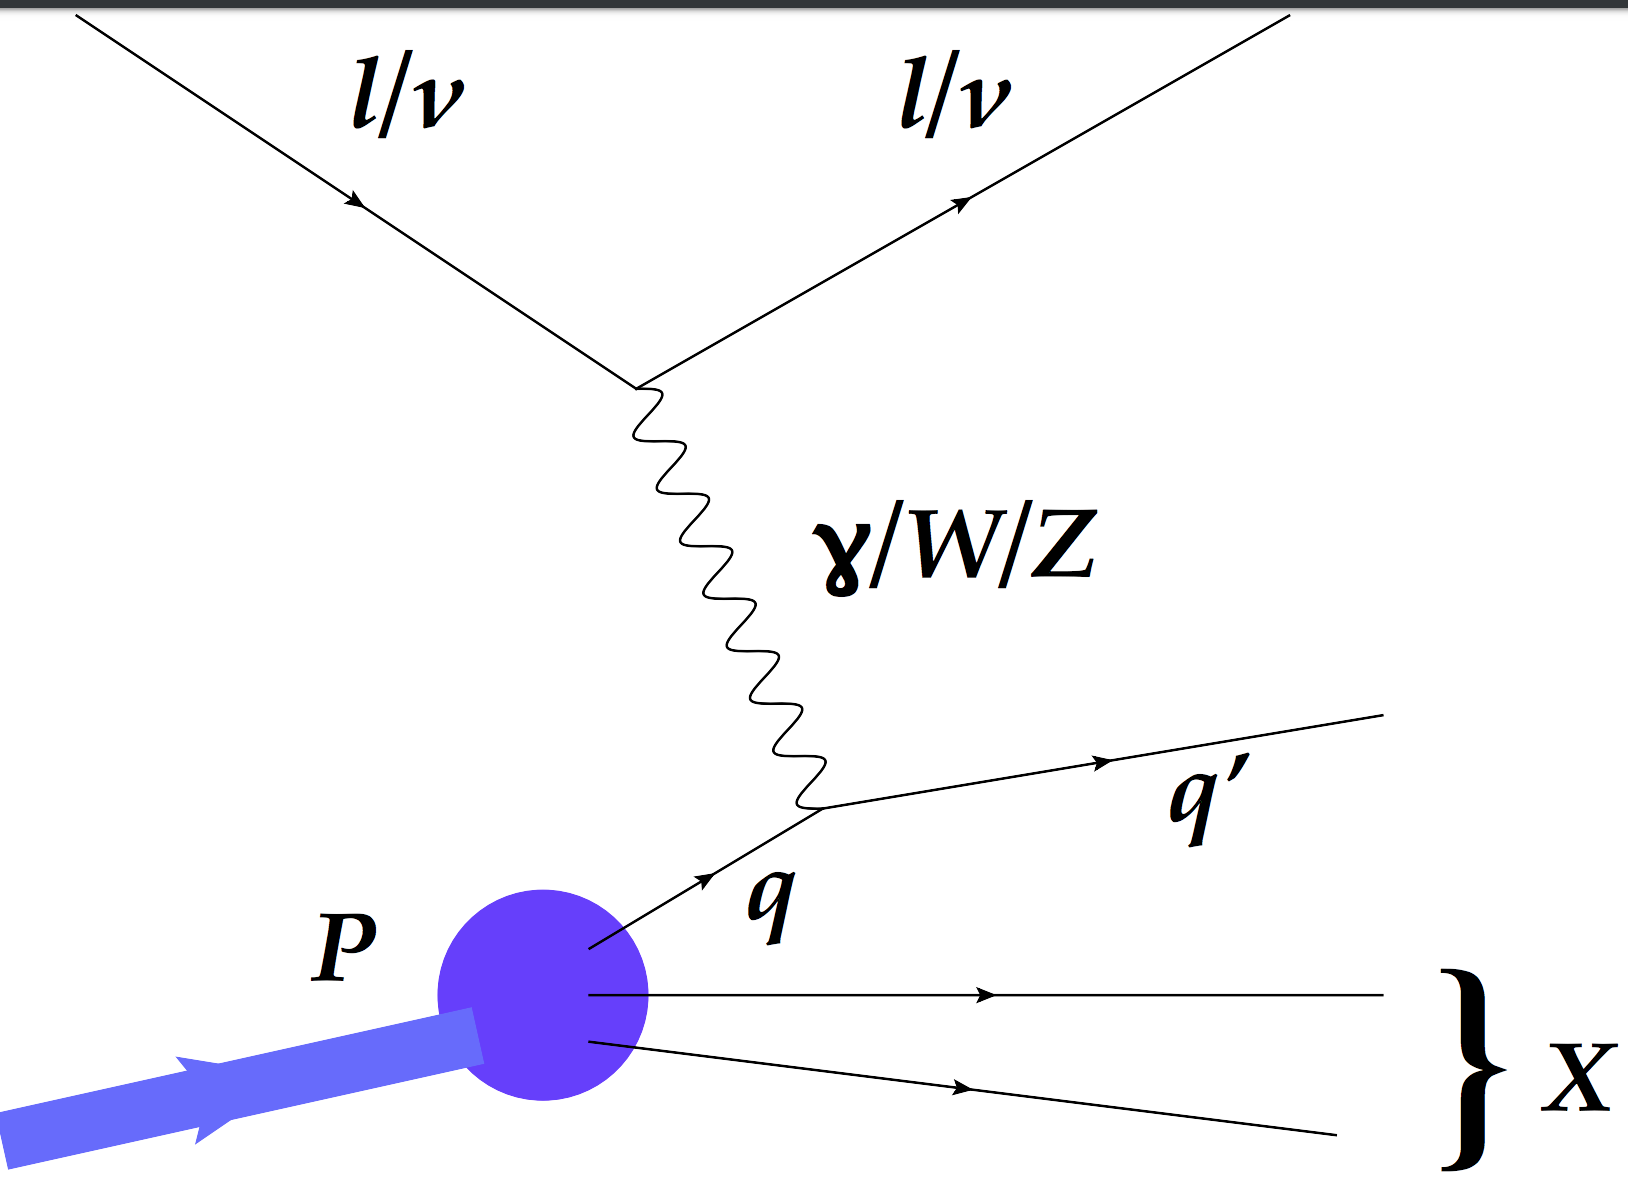
\includegraphics[width=\textwidth,keepaspectratio]{DIS.png}
				\caption[Side view]{DIS diagram~\cite{proton_struct}.}
				\label{fig::dis}
			\end{subfigure}
			\hfill
			\caption{Examples of hard QCD scatterings.}
			\label{fig::hadron_qcd}
		\end{figure}
		\subsection{Deep Inelastic scattering}
		In order to better illustrate the factorization approach let us first consider the lepton-hadron process called the \gls{dis}. Historically it was the first experimental evidence for the complex structure of the proton and still serves as an indispensable tool for the proton structure study. Let's try to write a matrix element for a \gls{dis} process $e+A\rightarrow e+X$, exchanging a virtual photon with momentum $q^{\mu}$:
		 \begin{equation}
		|M|^2_{DIS}=4\pi M_N\frac{\alpha}{q^4}L_{\mu \nu}W^{\mu \nu}_{hadron},
		\end{equation}
		where $L_{\mu \nu}$ is the transverse lepton tensor, $q^{\mu}L_{\mu \nu}=q^{\nu}L_{\mu \nu}=0$. The hadronic tensor $W_{\mu \nu}$ along with its normalization factor $4\pi M_N$ is unknown, but we can write it down in general form introducing longitudinal and transverse parts\footnote{Given example assumes only electromagnetic interaction. For the more general electroweak case the tensor structure is more complicated and there are more than two scalar structure functions \cite{proton_struct}.} \cite{factorization}:
		\begin{equation}
		W_{\mu \nu}=F_1(x,Q^2)\left(-g_{\mu \nu}+\frac{q_{\mu}q_{\nu}}{q^2}\right)+F_2(x,Q^2)\frac{\left(p_{\mu}-q_{\mu}p\cdot q / q^2\right)\left(p_{\nu}-q_{\nu}p\cdot q / q^2\right)}{p\cdot q},
		\end{equation}
		with $p_{\mu}$ being the momentum of the hadron A, $Q^2$ is the exchange momentum, $x=\frac{Q^2}{2p \cdot q }$ and the form-factor functions $F_1(x,Q^2)$, $F_2(x,Q^2)$ are unknown. \\
		The cross-section of the \gls{dis} process can be measured experimentally, leaving the possibility to study the form-factor functions. It turned out that these functions do not depend (at least in the first approximation) on $Q^2$ \cite{dis1}. Further experiments have revealed that the form-factors depend only on the ratio $x$, as it was predicted before \cite{bjorken}. This type of behaviour was called the Bjorken scaling.\\
		These results have led to the idea of partons - point-like constituents of the proton \cite{feynman_partons}. The factorization theorem states that it is possible to express the hadronic tensor $W_{\mu \nu}$ as a sum of all available partons:
			\begin{equation}
		W_{\mu \nu}(q_{\mu},p_{\nu})=\sum_{a} \int_{x}^{1}\frac{d\xi}{\xi} f_{a/A}(\xi,\mu) H^a_{\mu\nu}(q_{\mu},p_{\nu},\mu,\alpha_s(\mu)) + NLO.
		\end{equation}
		The functions $H^a_{\mu\nu}(q_{\mu},p_{\nu},\mu,\alpha_s(\mu))$ are called the hard scattering structure functions and only depend on parton type $a$, but not on hadron type $A$. These functions describe the high-energy behaviour and can be calculated in the framework of perturbative QCD. At the same time $f_{a/A}(\xi,\mu)$ is called \gls{pdf} and has a physical meaning of finding a parton of type $a$ (gluon, u-quark, d-quark etc ) in a hadron of type $A$ (proton, neutron, meson) carrying the fraction of $\xi$ of the hadron's momentum. These \gls{pdf}s contain information on the momentum distribution of quarks and gluons within the hadron. This corresponds to the non-perturbative sector of the QCD which is beyond the reach of theoretical methods available so far. Note that they do not directly depend on the momentum $Q^2$, but only on the energy scale $\mu$. \\
		The \gls{dglap} equations show that once the \gls{pdf}s are known at a certain energy scale $\mu$ they can be perturbatively extrapolated to a different energy scale \cite{Lipatov:1974qm}, \cite{ALTARELLI}, \cite{Gribov:1972ri}, \cite{Dokshitzer:1977sg}. The \gls{pdf}s are universal - they can be measured experimentally at certain conditions in the course of the DIS (or any other) process and then used for numerical calculations of any other process (e.g. \gls{dy} process) at different conditions. Such a measurement allows a workaround - we may not be able to solve the many-body problem and perform non-perturbative calculations starting from the first principles, yet we still get a theoretical prediction with a good precision. Currently there exists a number of different groups working on the PDF parametrizations and fits, constantly improving the fits using the data coming from hadron and electron-proton colliders. Using different PDF sets may give different results and also helps to estimate the systematic uncertainties implied by the PDFs. \\
		Historically the DIS experiments at HERA electron-proton collider have allowed to perform proton PDFs measurements with a good level of precision in the $x$ region up to $x \backsim 10^{-4}$ at high $Q^2$ of up to 50 000 $GeV^2$~\cite{shushin}. The HERA experiments operated until 2008, paving the path for precision predictions for the Drell-Yan process.  Currently there are prospects for new experiments like \gls{lhec} that would involve DIS and further improve the PDF precision \cite{lhec}.
		\begin{figure}[htbp]
		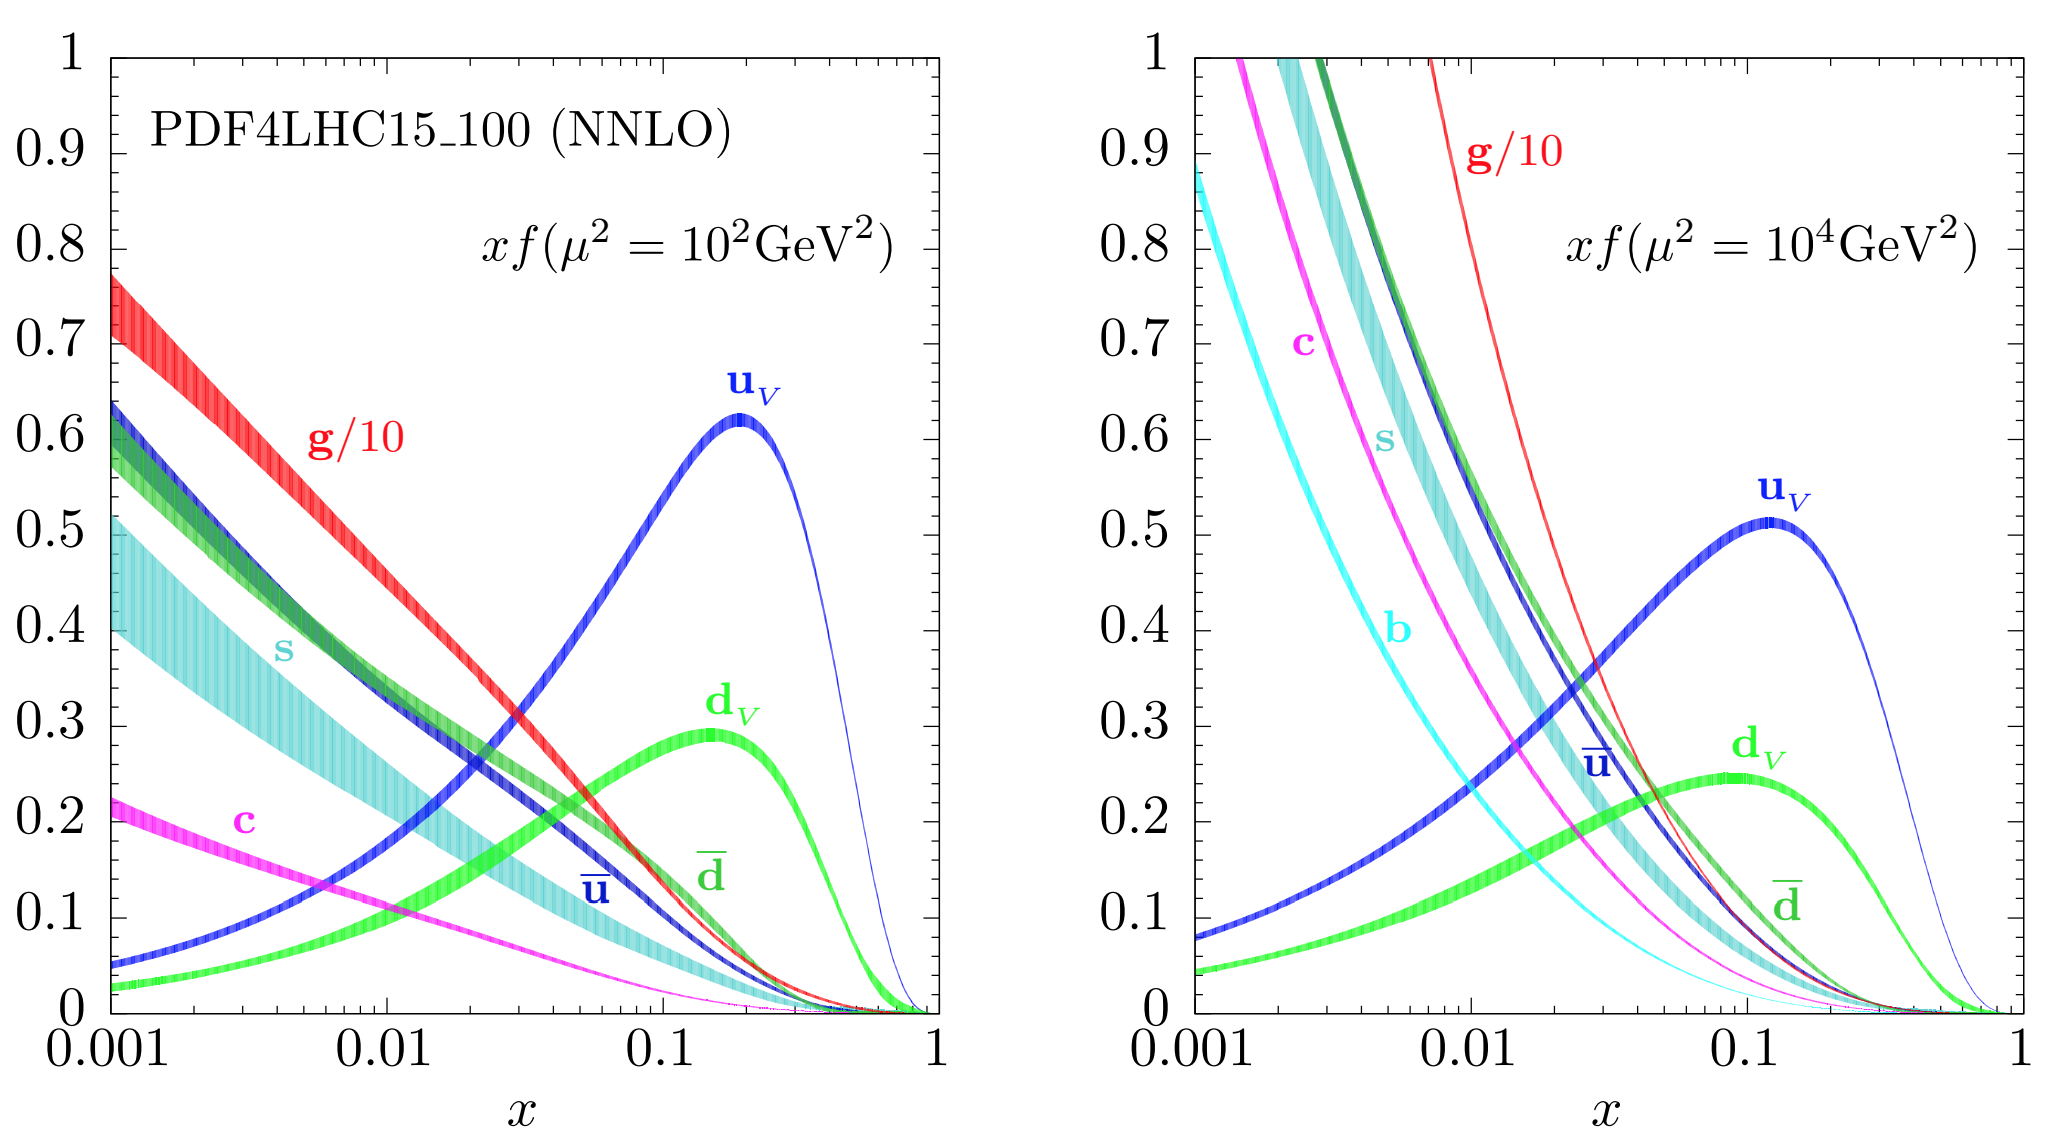
\includegraphics[width=\textwidth,keepaspectratio]{pdfs.png}
		\caption{The evolution of a PDF4LHC15 NNLO Hessian set from $Q^2=10^2$ GeV to $Q^2=10^4$ GeV using the \gls{dglap}. Notice the increase in the sea quark density. The PDFs include one standard deviation uncertainty band~\cite{proton_struct}.}
		\label{fig::pdfs}
		\end{figure}
 		\subsection{The Drell-Yan process}
		The \gls{dy} process happens during the high-energy hadron-hadron scattering when quark and antiquark annihilate to form an electroweak boson~\cite{drellyan}. For the neutral DY process $q\bar q \rightarrow Z/\gamma^* + X \rightarrow l^{+}l^{-} + X$ takes place. In a similar way the charged DY process can happen, generating a W boson: $ q\bar q' \rightarrow W^{\pm} +X \rightarrow l^{\pm}\nu + X$. It is postulated that the \gls{dy} cross-section $\sigma^{DY} $ in a proton-proton scattering  can be expressed through the cross-sections of the corresponding parton-parton scattering cross-section convoluted with the \gls{pdf}s of these partons:
		\begin{equation}
		\frac{d^2\sigma^{DY}}{dydM^2}=\sum_{a,b=q,\bar q,g}\int_{\tau_1}^1 dx_1 f_a(x_1,\mu_F^2) \int_{\tau_2}^1 dx_2 f_b(x_2,\mu_F^2)\frac{d^2\hat{\sigma}_{ab}^{DY}}{dydM^2}(x_1,x_2,y,M^2,\mu_R^2,\mu_F^2).
		\label{eq::diffY}
		\end{equation}
		In this equation $y=\frac{1}{2}\log{\frac{E+p_z}{E-p_z}}$ represents rapidity, $M^2$ is the invariant mass of the lepton pair, $\mu_F$ and $\mu_R$ are factorization and renormalisation scales correspondingly. Integration limits $\tau_{1,2}=\sqrt{\frac{Q^2}{s}}e^{\pm y}$ with $s$ being the centre-of-mass energy of the two incoming protons. The partonic cross-sections can be in turn computed perturbatively as a series expansion in $\alpha_s$ \cite{proton_struct}:
		\begin{equation}
		\frac{d^2\hat{\sigma}_{ab}^{DY}}{dydM^2}(x_1,x_2,y,M^2,\mu_R^2,\mu_F^2)=\sum_{n=0}^{\infty}\left(\frac{\alpha_s\mu^2_R}{2\pi}\right)^{(n)}\frac{d^2\hat{\sigma}_{ab}^{(n)DY}}{dydM^2}.
		\end{equation}
		The cross-sections $\hat{\sigma}_{ab}^{(n)DY} \propto \alpha_s^n$ contain only the terms of order $n$ in $\alpha_s$. 
		The exact sum of the expansion does not depend on the $\mu_F$ and $\mu_R$ parameters. However, finite-order calculations demand a specific choice for the two parameters. One of the common choices for the \gls{dy} process is putting  $\mu_F=\mu_R=M$, with $M$ being the mass of the dilepton pair. \\
		From equation \ref{eq::diffY} we can see that the rapidity distribution of the vector boson explicitly depends on the \gls{pdf}s both in terms of flavour decomposition and in the sense of a particular PDF set. Figure \ref{fig::Wrapidity} demonstrates different rapidity distributions for two centre-of-mass energies and two different PDF sets.\\
		\begin{figure}[htbp]
			\centering
			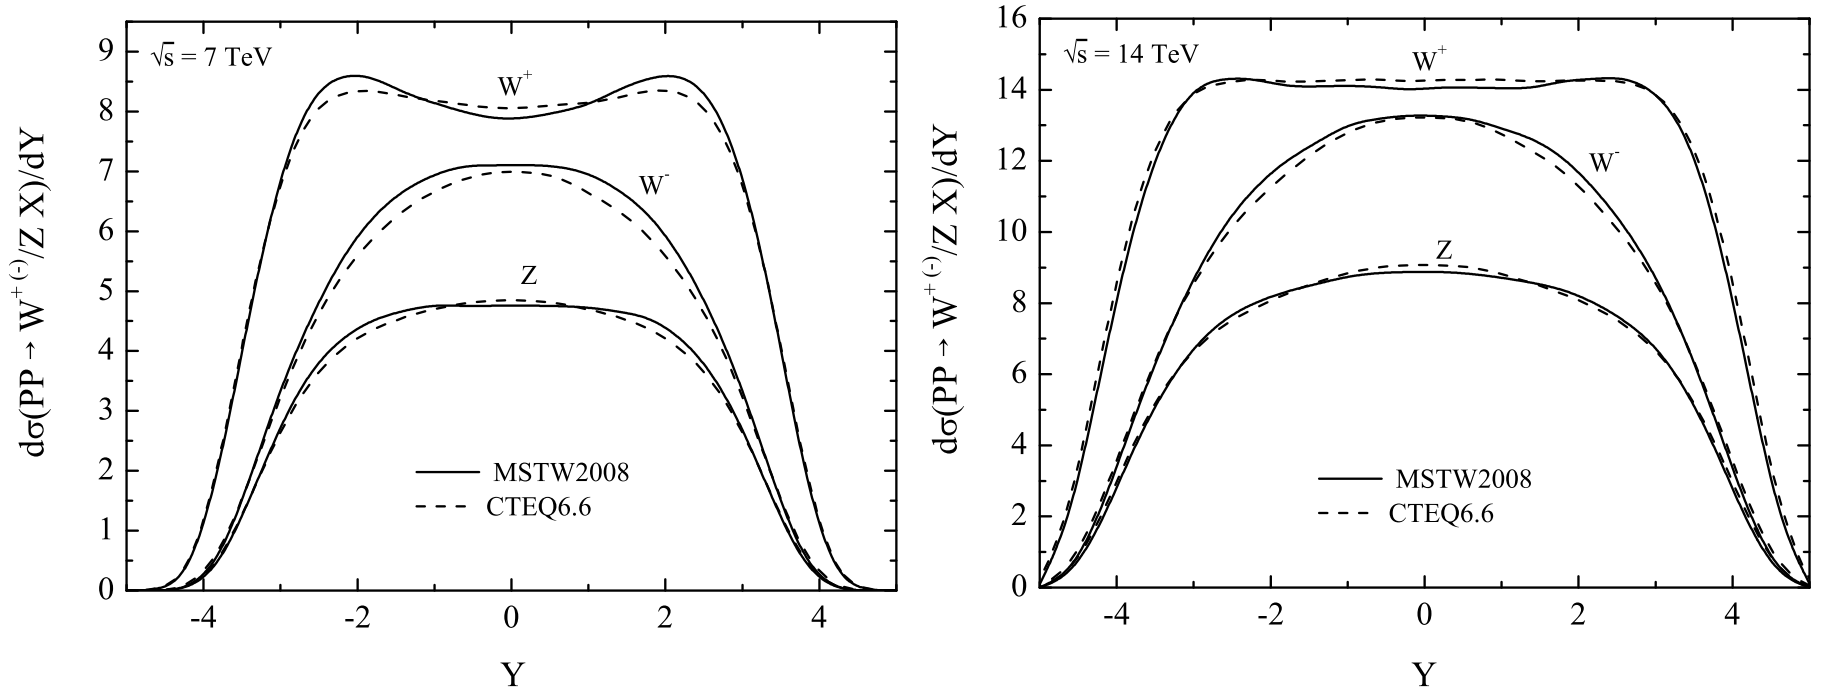
\includegraphics[width=\textwidth,keepaspectratio]{rapidity.png}
			\caption{ Rapidity distribution for the vector bosons using MSTW2008 and CTEQ6.6 PDF sets for the centre-of-mass energies of 7 and 14 TeV \cite{Halzen:2013bqa}.}
			\label{fig::Wrapidity}
		\end{figure}
		Let us consider partonic cross-sections, which can be constructed using an analogy to QED $e^{+}e^{-}\rightarrow \mu^{+}\mu^{-}$:
		\begin{equation}
			\hat{\sigma}(q\bar q \rightarrow e^{+}e^{-}) = \frac{4\pi \alpha^2}{3s}\frac{1}{N}Q^2_q.
		\end{equation}	
		Here $Q_q$ is the quark charge, $1/N$ stands for the averaging over colour factor and underlines the fact that quark and antiquark must have the matching colour in order to annihilate. In a similar way we can obtain the cross-section of the sub-processes of W and Z bosons production:

		\begin{equation}
		\begin{array}{lcl} 
		\hat{\sigma}^{q\bar q^\prime \rightarrow W}= \frac{\pi }{3}\sqrt{2}G_FM^2_W|V_{qq^\prime}|^2\delta(s-M^2_W),\\
		\hat{\sigma}^{q\bar q^\prime \rightarrow Z}= \frac{\pi }{3}\sqrt{2}G_FM^2_W(v^2_q+a^2_q)\delta(s-M^2_Z),
		\end{array}
		\end{equation}	
		where $V_{qq^\prime}$ is the element of the \gls{ckm} matrix,  $v_q$ ($a_q$) is a vector (axial vector) that couples the Z boson to the quarks. Figure \ref{fig::wxsec} shows the contributions of different parton flavours into $W^+$ and $W^-$ cross-sections. An assumption of narrow W resonance was used. The fact that the bosons with opposite charges are formed from different quarks makes a notable difference at the LHC experiments. Figure \ref{fig::wzxsec} contains the comparison of the results obtained at the LHC experiments with the NNLO theoretical predictions that use different PDF sets.
		\begin{figure}[htbp]
			\centering
			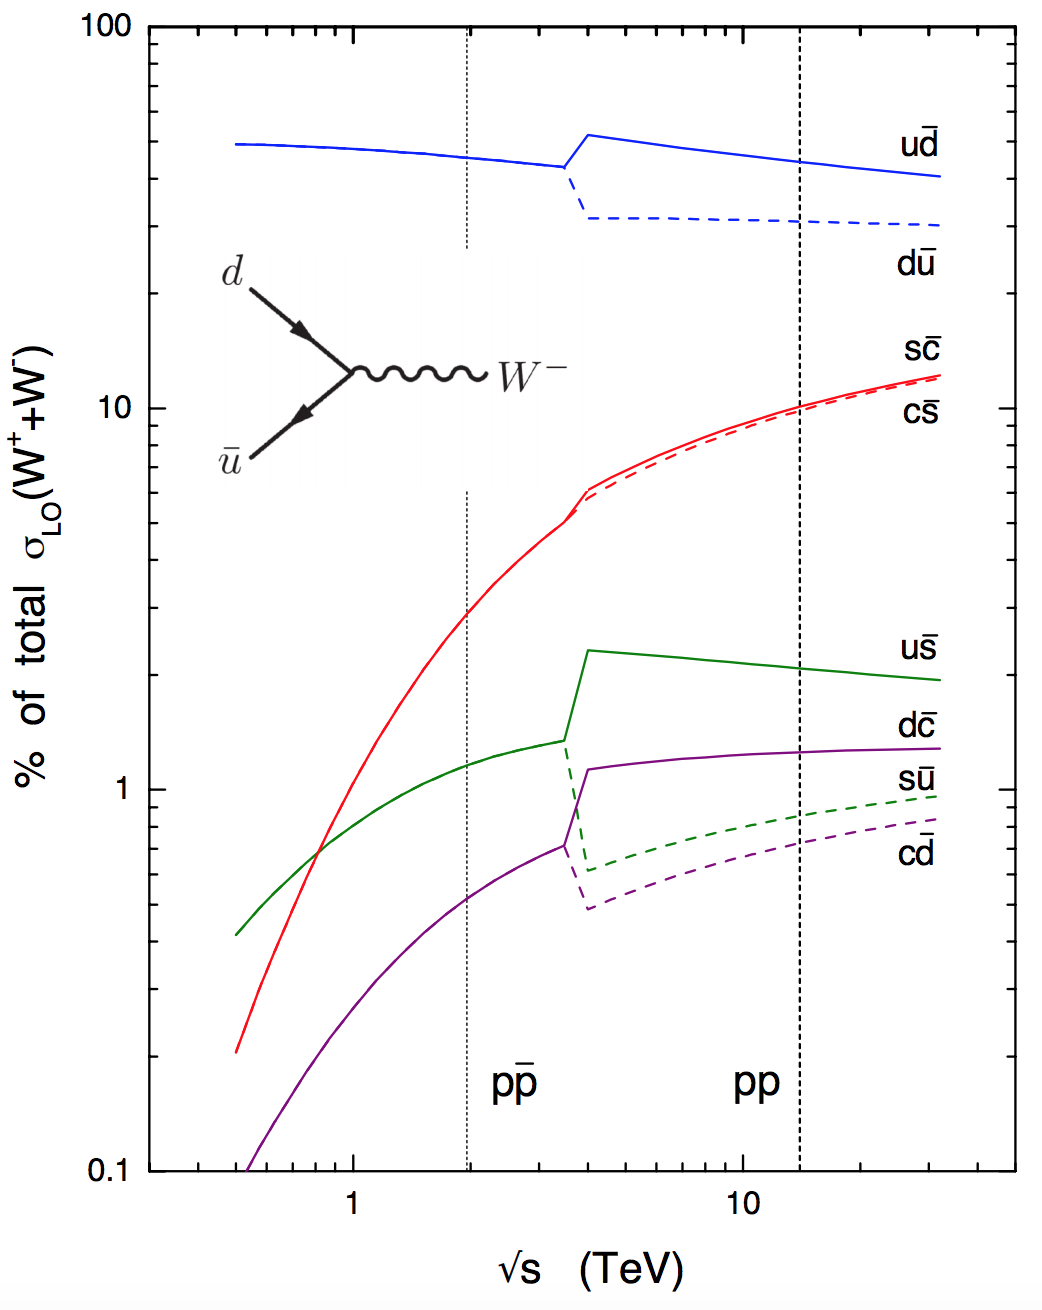
\includegraphics[width=0.5\textwidth,keepaspectratio]{wxsec1.png}
			\caption{Parton contributions to the cross-sections of $W^+$ and $W^-$ bosons for LHC and Tevatron cases \cite{Martin:392675}.}
			\label{fig::wxsec}
		\end{figure}
		\begin{figure}[htbp]
		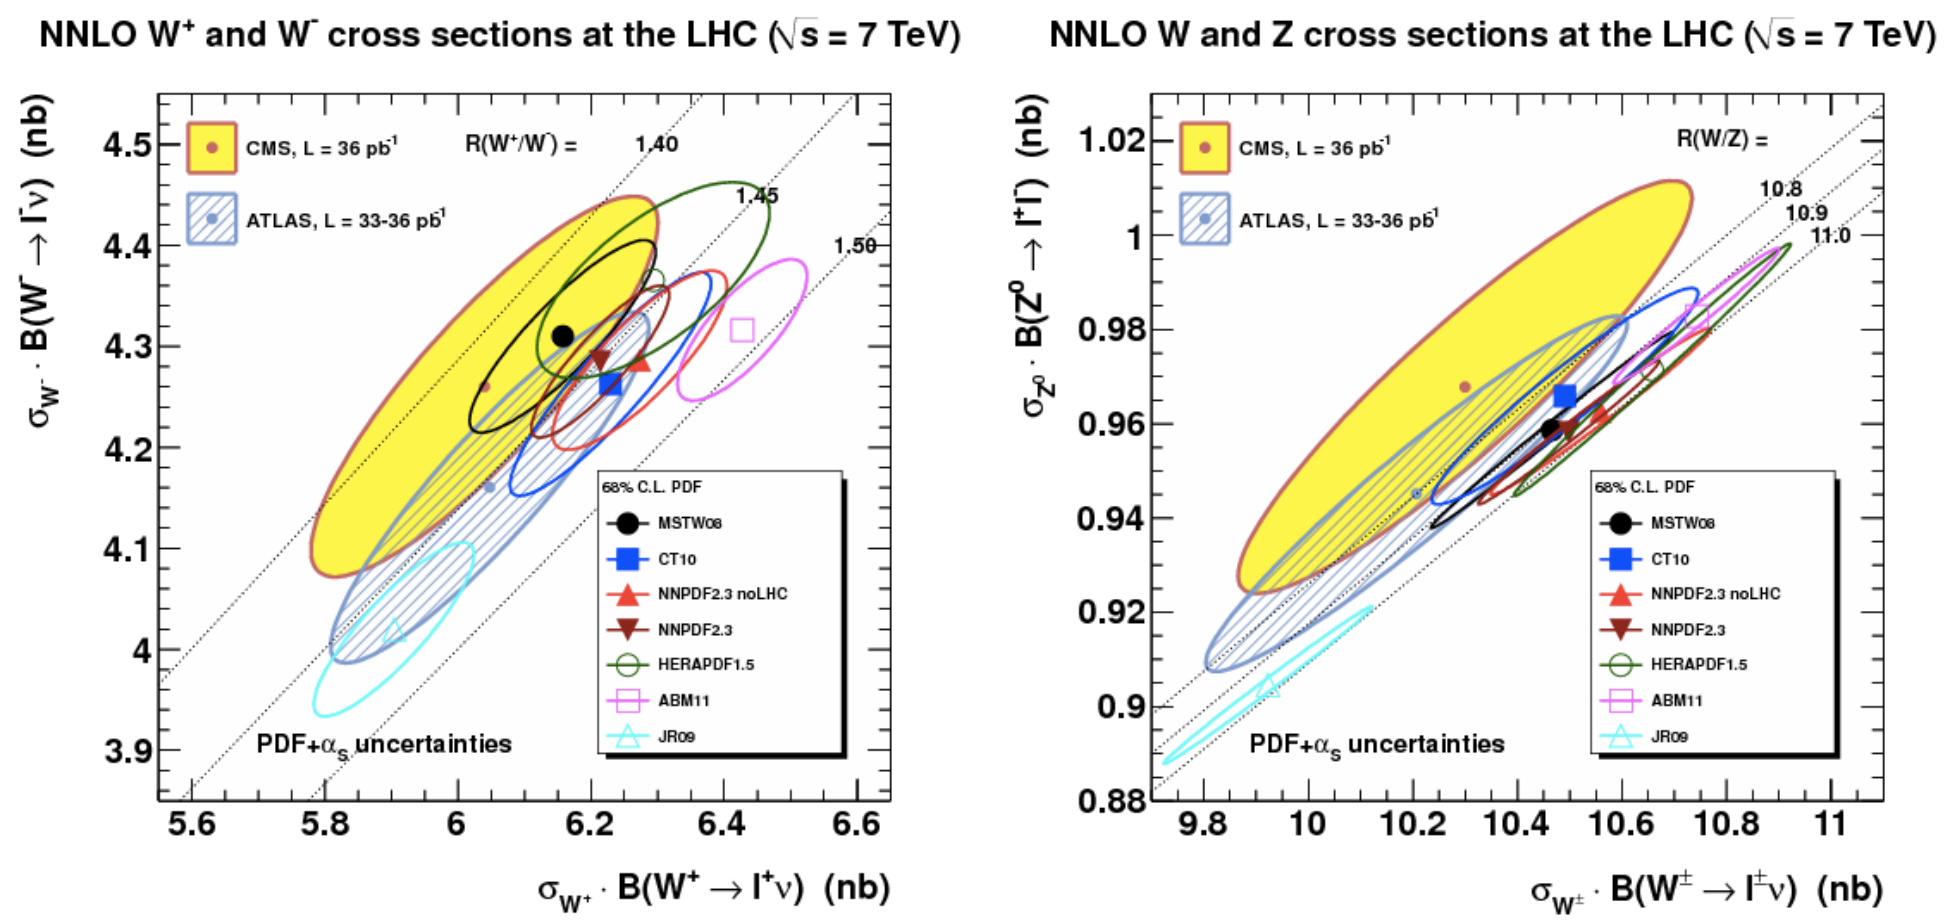
\includegraphics[width=\textwidth,keepaspectratio]{WZxsec.png}
		\caption{W and Z boson cross sections LHC at 7 TeV. ATLAS and CMS results, compared to NNLO predictions for various PDF sets \cite{Mangano:2015ejw}.}
		\label{fig::wzxsec}
		\end{figure}

	
		 \section{Transverse momentum of massive vector bosons }
		 The leading-order model of the \gls{dy} process assumes the colliding partons to have their momentum perfectly collinear with the proton as a whole, which would mean that the vector boson $p_T$ should peak at zero. However most of the massive vector bosons produced in the \gls{dy} process have a small yet non-zero transverse momentum, $p_T \ll M_V$. The main source for the W boson transverse momentum is the initial state radiation by one of the two quarks that create the boson.
		 The spectrum at higher values of $p_T$ is determined by hard perturbative parton emission(s) like $q\bar q \rightarrow Vg$, $qg \rightarrow Vq$. The corresponding amplitudes can be conveniently expressed using Mandelstam variables:
	\begin{equation}
	\begin{array}{lcl} 
	\label{eq::xsec_nlo}
		 \sum |\mathcal{M}^{q\bar q'\rightarrow Wg}|^2= \alpha_s \sqrt{2}\pi G_F M^2_W |V_{q\bar q'}|^2 \frac{8}{9}\frac{t^2+u^2+2M_W^2s}{tu},\\
		 \sum |\mathcal{M}^{qg\rightarrow Wq'}|^2= \alpha_s \sqrt{2}\pi G_F M^2_W |V_{q\bar q'}|^2 \frac{1}{3}\frac{s^2+u^2+2M_W^2t}{-su},
		 \end{array}
	 \end{equation}	
	 where the summation is performed over colours and spins in the final and initial states. Integrating these partonic matrix elements with the \gls{pdf}s one can obtain the transverse momentum distribution $d\sigma/dp_T$. Further precision can be obtained by considering corrections from next-to-leading order processes $\backsim O(\alpha_s^2)$ like $q \bar q \rightarrow Vgg$ - that would mainly affect the high $p_T$ tail of the distribution. \\
	 The matrix elements in \ref{eq::xsec_nlo} become singular when the emitted partons become soft or collinear to the initial-state partons - it is related to the poles at $u=0$ and $t = 0$ in the denominator. Also for the NLO processes like $q \bar q \rightarrow Vgg$ a singularity arises if the two final-state gluons are collinear. This creates a problem for the calculation of the low-$p_T$ part of the spectrum. Mathematically it is reflected in the appearance of different powers of logarithms like $\log{M^2_W/p^2_T}$ in all orders of cross-section expansion in $\alpha_s$, which leads to divergences when $p_T$ is small. This forces us to look for alternative approach that would take into account all the orders of the expansion.\\
	 All-order resummation may be performed in a variety of approaches, one of the most popular is provided by parton showers. Its numerical implementation is available in a number of Monte-Carlo generators, PYTHIA, HERWIG and SHERPA are among the most used. It appears that for the case of soft and collinear gluon emission it is possible to factorize and exponentiate the logarithms in a \textit{Sudakov form factor}, such that:
	 	\begin{equation}
	 		\begin{array}{lcl} 
		\frac{d\sigma}{dp_T^2}=\sigma\frac{d}{dp_T^2}\exp{-\frac{\alpha_s C_F}{2\pi}\log^2{\frac{M_W^2}{p_T^2}}},\\
		\exp{-\frac{\alpha_s C_F}{2\pi}\log^2{\frac{M_W^2}{p_T^2}}}=1-\frac{\alpha_s}{2\pi}C_F\ln^2{\frac{M_W^2}{p_T^2}}+\frac{1}{2!}\left(\frac{\alpha_s}{2\pi}\right)^2C^2_F\ln^4{\frac{M_W^2}{p_T^2}}-\frac{1}{3!}\left(\frac{\alpha_s}{2\pi}\right)^3C^3_F\ln^6{\frac{M_W^2}{p_T^2}}+...
				 \end{array}
	 \end{equation}	
	 The exponential $\exp{G(\alpha_s,L)}$, where $L=\log{M^2_W/p^2_T}$ is called the Sudakov form-factor. Its expansion by the powers of $\alpha_s$ defines the resummation accuracy: the term $\backsim O(\alpha_s)$ is called the leading logarithm (LL), term with $ \backsim O(\alpha_s^2)$ is the next-to-leading logarithm (NLL) and so on. \\
	 The cross-sections obtained with the resummation methods provide a good prediction for soft and collinear emissions at low $p_T\ll M_W$. In order to get a combined cross-section for higher $p_T$ region the resummed cross-section has to be \textit{matched} with the fixed-order cross-sections of the corresponding power in $\alpha_s$. Figure \ref{fig::w_kinematics} contains NNLO resummed predictions for the W $p_T$ spectrum produced with RadISH\cite{Radish}. In Chapter 9 of this thesis the spectrum generated by another resumming tool - DYRes~\cite{dyres}, is used for comparison with \Powheg and \Sherpa predictions.
	 \begin{figure}[htbp]
	 	\begin{subfigure}[t]{0.31\textwidth} 
	 		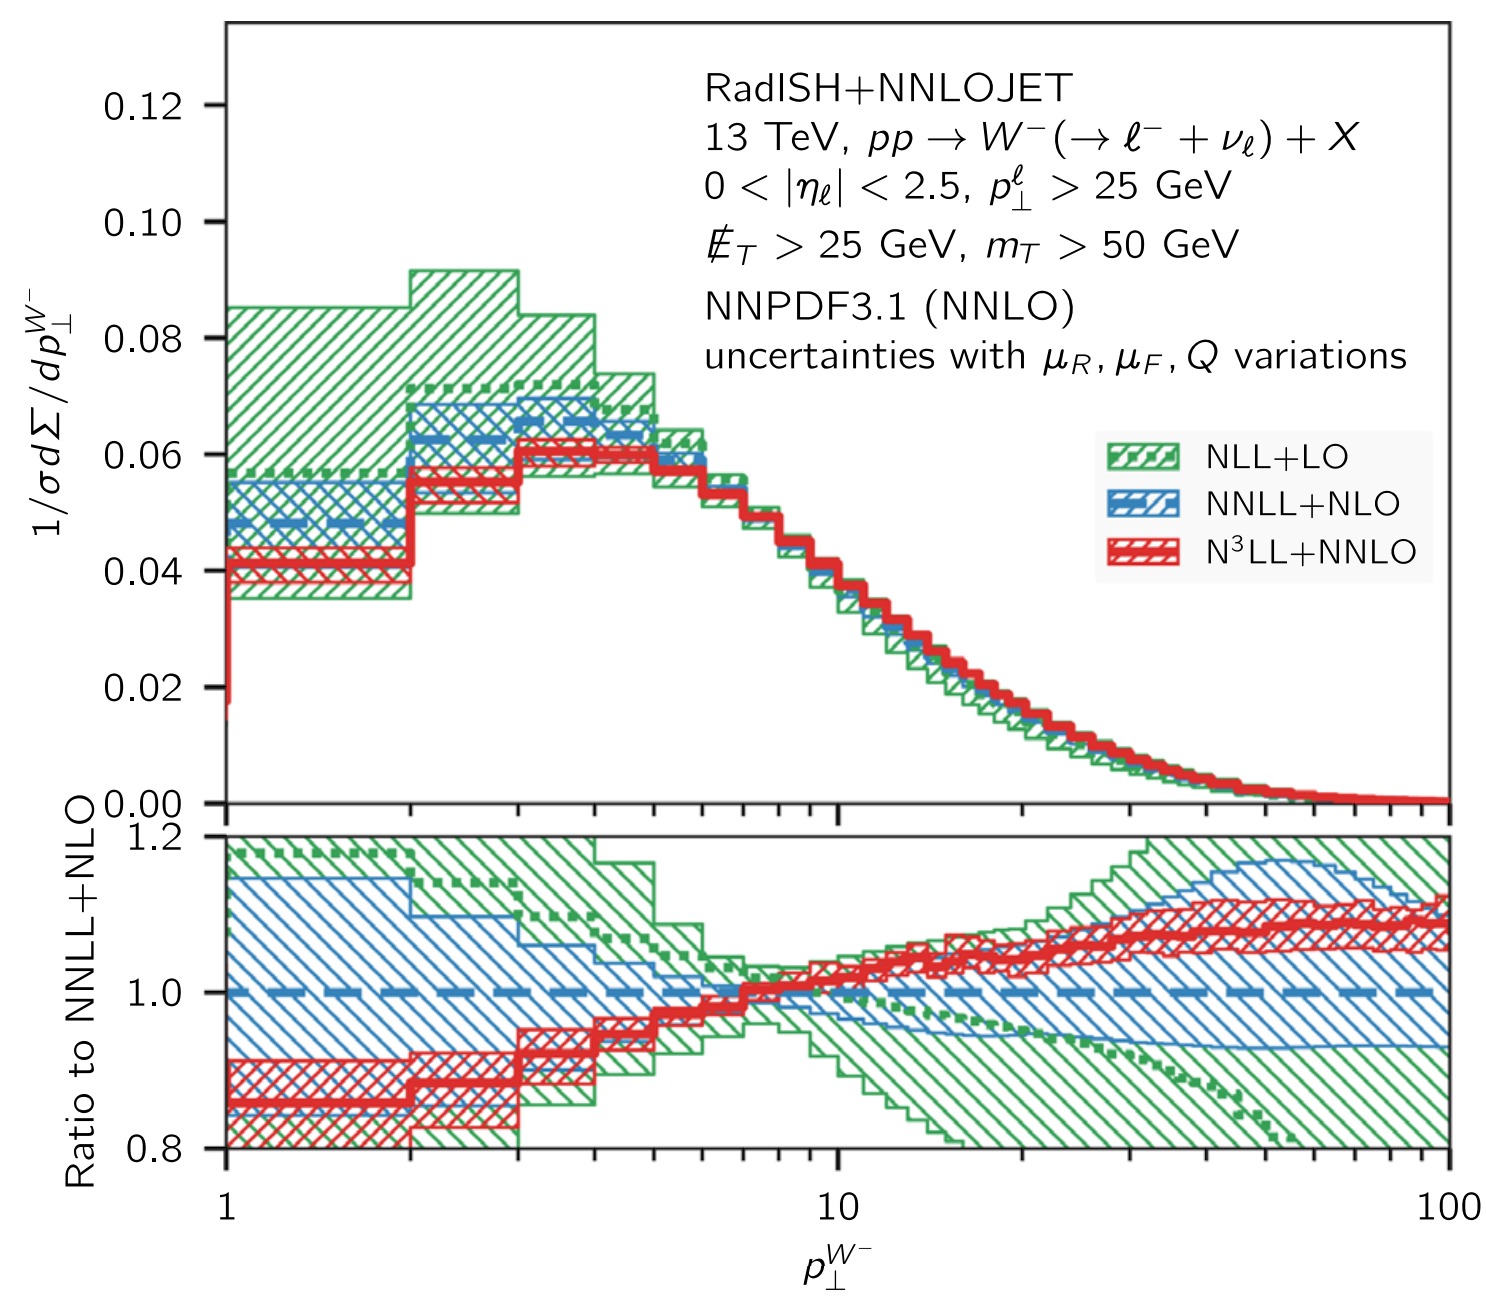
\includegraphics[width=\textwidth,keepaspectratio]{pt_nlo_wm.png}
	 		\caption[Transverse view]{$W^{-}$ transverse momentum spectrum \cite{Bizon:2019zgf}.}
	 		\label{fig::wm_pt}
	 	\end{subfigure}
	 	\begin{subfigure}[t]{0.31\textwidth}
	 		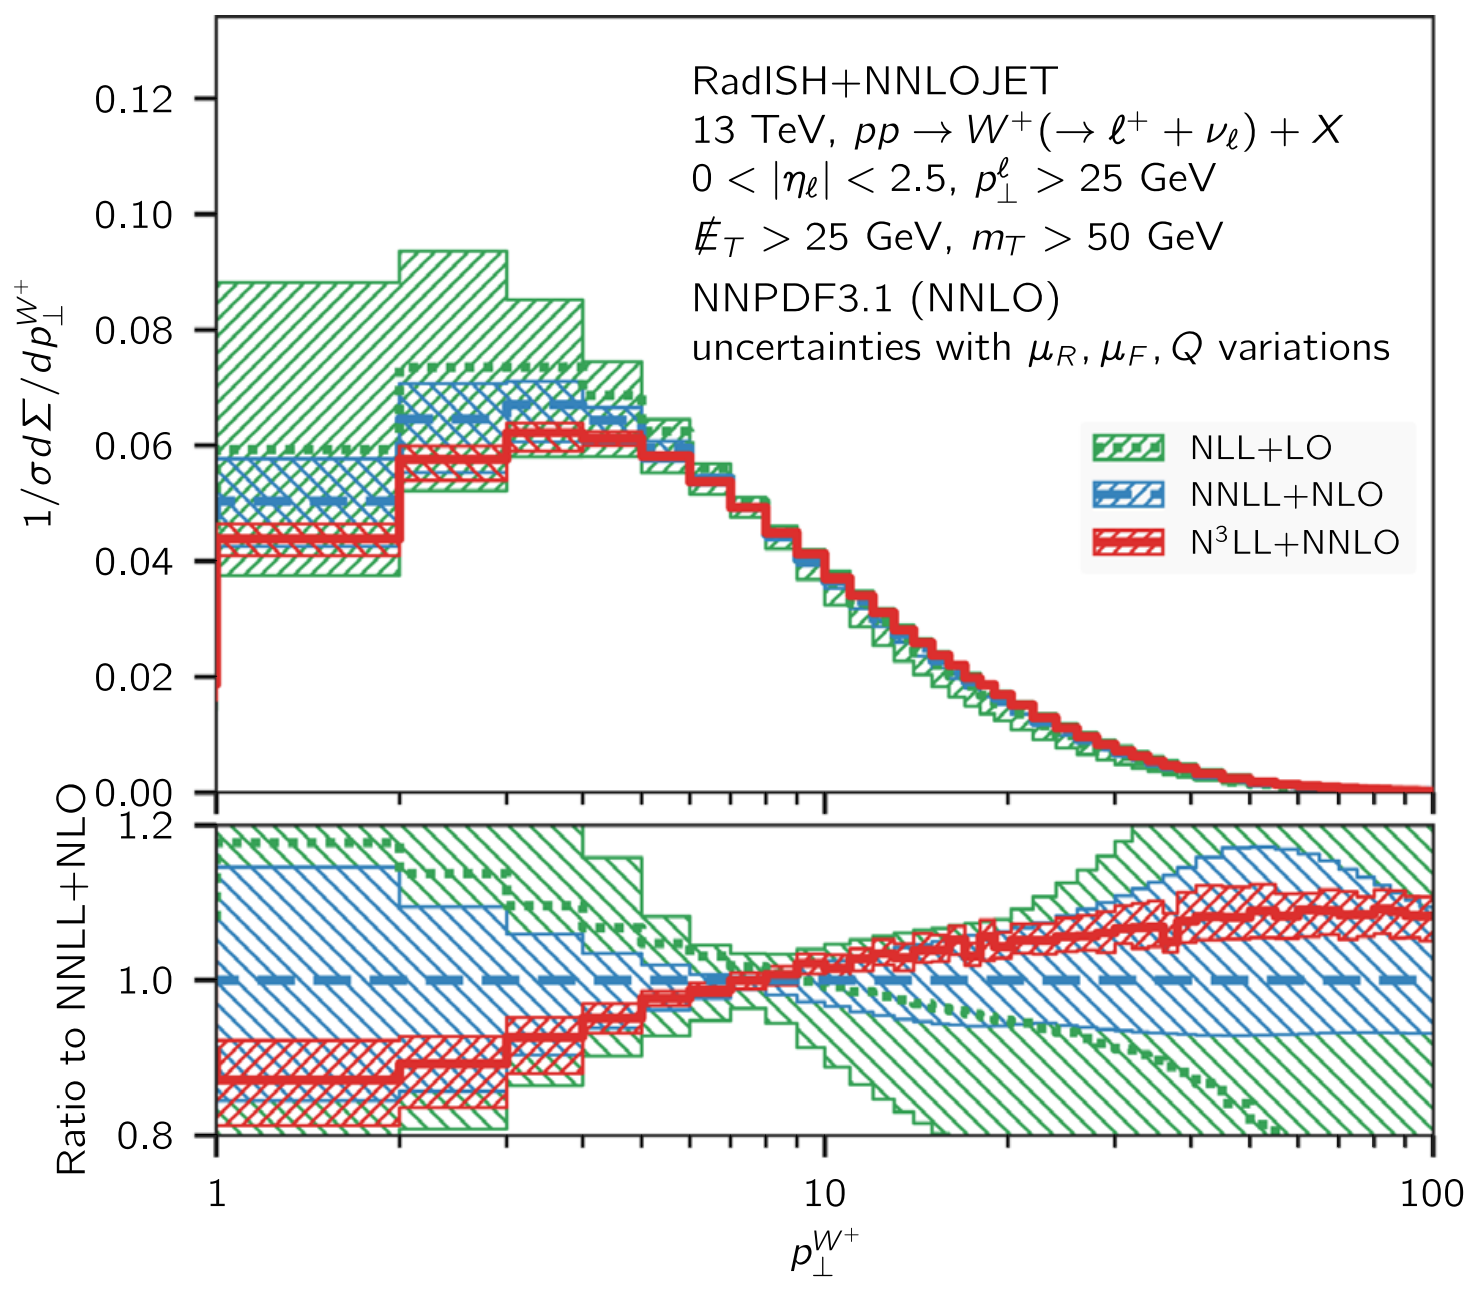
\includegraphics[width=\textwidth,keepaspectratio]{pt_nlo_wp.png}
	 		\caption[Side view]{$W^{+}$ transverse momentum spectrum \cite{Bizon:2019zgf}.}
	 		\label{fig::wp_pt}
	 	\end{subfigure}
	 	\hfill
	 		\begin{subfigure}[t]{0.36\textwidth}
	 		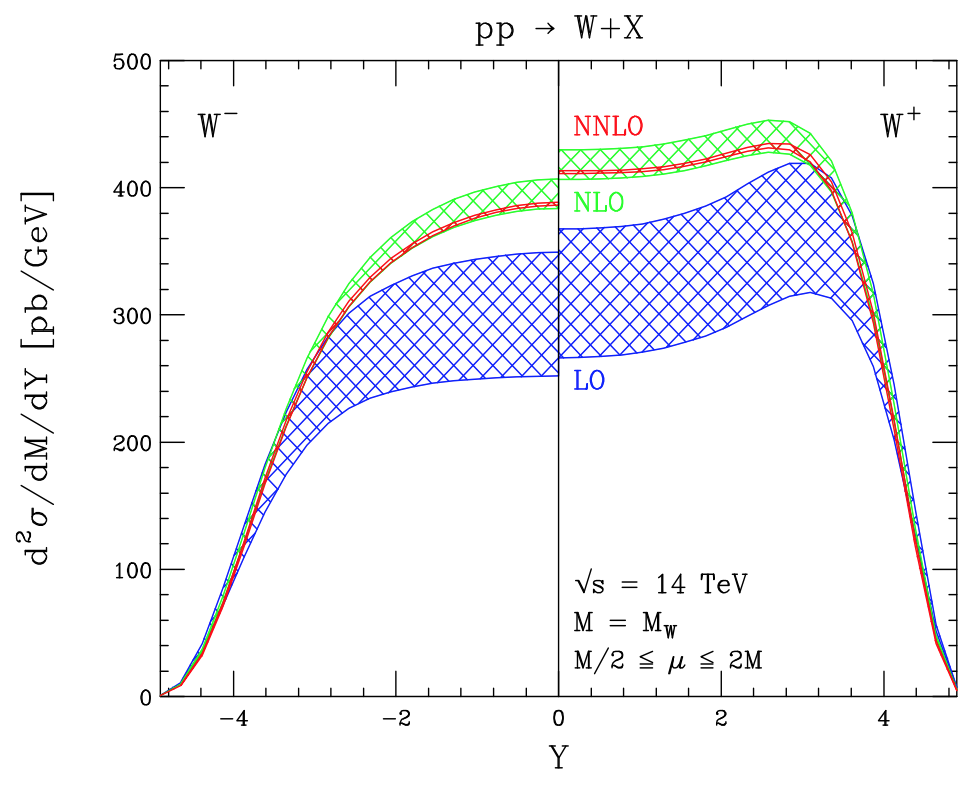
\includegraphics[width=\textwidth,keepaspectratio]{rapidity_nlo.png}
	 		\caption[Side view]{$W^{\pm}$ rapidity distribution \cite{Anastasiou:2003ds}.}
	 		\label{fig::w_rapid}
	 	\end{subfigure}
	 	\caption{Kinematic distributions for $W^{\pm}$ with corrections.}
	 	\label{fig::w_kinematics}
	 \end{figure}
 Besides the ISR phenomena, there is also an effect of partons moving within the colliding protons, having an intrinsic momentum of their own. This intrinsic momentum $<k_T>\backsim \Lambda_{QCD}$ is well parametrized using a Gaussian distribution with average value of $500$ \cite{PhysRevD.100.074027} or $700$ MeV  \cite{Ellis:1991qj}, although there are ongoing efforts for a more sophisticated parametrization that would allow a better modelling of the lower part of vector boson spectrum, at $p_T<2\gev$~\cite{HAUTMANN2020135478}. \\
 
 
\section{The measurement of W boson transverse momentum}
As it was shown in Fig. \ref{fig::w_kinematics} the shape of the W transverse momentum distribution is a difficult problem from the theoretical point of view. It heavily depends on the level of theoretical precision and the resummation technique. This is particularly illustrated by the fact that the predictions from different MC generators often do not agree (see, for instance, Figures \ref{fig:results_predictions_elec} and \ref{fig:results_predictions_muon}). In this situation a precise measurement would help benchmarking the MC predictions and also test our understanding of the Standard Model.

The measurement of the W boson transverse momentum at hadron colliders is a complicated problem. The hadronic decay channels can not be used for the measurement as such decay are very hard to discriminate from the QCD background. The leptonic decays have a clear signature and allow for efficient background rejection, although due to the presence of a neutrino in the final state there is no possibility to measure the transverse momentum spectrum from the final states, like in the $Z\rightarrow l^+ l^-$ case.

As it was described in the previous section, the transverse momentum spectrum of vector bosons is caused by the initial state radiation (ISR). The partons produced as a result of the ISR compensate the transverse momentum of the boson. Measuring the combined momentum of these partons allows to reconstruct the vector boson momentum: $\vec{p_T}^{V} = -\sum \vec{p_T}^{ISR}$. This effectively means the measurement of the transverse momentum of the hadronic final states of the ISR. The corresponding observable is called the hadronic recoil (HR) and is described in more detail in Chapter 7. 

The measurement of the HR is strongly dependent on the resolution of the ATLAS hadronic calorimeter. The resolution, in turn, depends on the level of noise in the calorimeter. The main sources of the noise are the pile-up (mean number of primary vertices per bunch crossing) and the underlying event. The right plot on Fig. \ref{fig:sigma_set} demonstrates a square root dependence between the calorimeter resolution and the sum of the transverse energies on all the objects in the event - $\sum E_T$. This quantity represents the combination of pile-up and underlying event activity. The plot on the right shows the dependence on pile-up and demonstrates two things: first, it is only possible to achieve a precision of 5-6 GeV and having a reasonable resolution of the spectrum peak if the pile-up is around $\langle \mu \rangle \approx 2$. That would also allow to use lower calorimeter threshold improving the resolution (calorimeter threshold is explained in more detail in Chapter 6).

	\begin{figure}[tph]
	\centering
	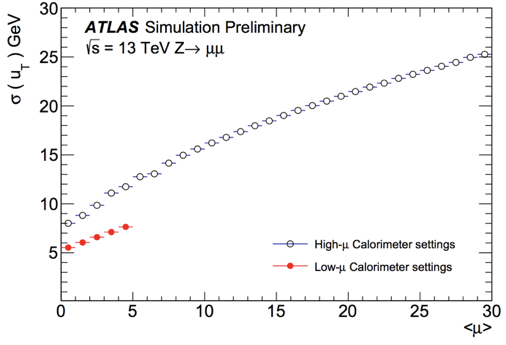
\includegraphics[width=.49\textwidth]{sigma_pileup}%
	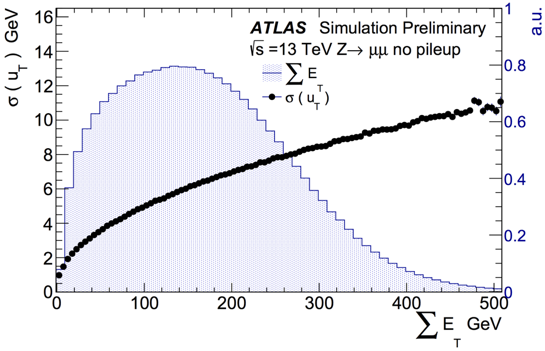
\includegraphics[width=.49\textwidth]{sigma_set}
	\caption{The dependence of the hadronic calorimeter resolution on pile-up (left) and on the soft event activity (right)~\cite{wpt_prospects}.}
	\label{fig:sigma_set}
	\end{figure} 

So far there were only two measurements of the W boson $p_T$ at the LHC: in ATLAS~\cite{wpt_atlas} and in CMS~\cite{wpt_cms}. Both measurements have used the data collected the special low pile-up runs, and both suffered from low statistics ($31~pb^{-1}$ for ATLAS and $18.4~pb^{-1}$ for CMS) that resulted in coarse binning (about 8 GeV at low $p_T$) and high relative uncertainties of about 2.5\% per bin.

Another strong motivation for a precise measurement of the W boson transverse momentum is its importance for the W boson mass measurement. W boson mass is extracted from the kinematic distributions that directly depend on the $p_T$ distribution of the W boson. 

For the Tevatron measurement of the W mass the position of the W boson transverse spectrum peak was taken from the Z $p_T$ spectrum, which was measured with good precision using the leptonic final states of the Z boson decay \cite{wmass_cdf}. However, this approach would lead to much higher uncertainties at the LHC energies due to significantly larger fraction of W bosons induced by the second generation quarks. 

The ATLAS measurement of the W boson mass has used the W $p_T$ extrapolated from the Z boson $p_T$ using the differential cross-section ratio:
		\begin{equation}
R_{W/Z}(p_T)=\left(\frac{1}{\sigma_W} \frac{d\sigma_W(p_T)}{dp_T} \right)\cdot\left(\frac{1}{\sigma_Z} \frac{d\sigma_Z(p_T)}{dp_T} \right)^{-1},
\end{equation}	
where the W $p_T$ cross-section was taken from the ATLAS 2011 measurement~\cite{wpt_atlas}. This has allowed to perform a very precise measurement of the W boson mass, although the $p_T$ spectrum extrapolation uncertainty turned out to be the second largest in the measurement reaching 8-9 GeV. The dominant PDF uncertainty has a comparable magnitude of 9-10 GeV, although it is expected to improve from the Drell-Yan process measurements to come. 

The goal for the new measurement of a W transverse momentum spectrum is to have a binning of around 5-6 GeV at low $p_T$ and a relative uncertainty of about 1\%. This would allow to reduce the QCD modelling uncertainty by as much as 50\%, significantly improving the W boson mass measurement precision~\cite{wpt_prospects}.